%%%%%%%%%%%%%%%%%%%%%%%%%%%%%%%%%%%%%%%%%
% Lightning presentation on using 
% freely available statistics to prove
% things "everyone knows" wrong.
%%%%%%%%%%%%%%%%%%%%%%%%%%%%%%%%%%%%%%%%%

%----------------------------------------------------------------------------------------
%	PACKAGES AND THEMES
%----------------------------------------------------------------------------------------

\documentclass{beamer}

\mode<presentation> {

% The Beamer class comes with a number of default slide themes
% which change the colors and layouts of slides. Below this is a list
% of all the themes, uncomment each in turn to see what they look like.

%\usetheme{default}
%\usetheme{AnnArbor}
%\usetheme{Antibes}
%\usetheme{Bergen}
%\usetheme{Berkeley}
%\usetheme{Berlin}
%\usetheme{Boadilla}
%\usetheme{CambridgeUS}
%\usetheme{Copenhagen}
%\usetheme{Darmstadt}
%\usetheme{Dresden}
%\usetheme{Frankfurt}
%\usetheme{Goettingen}
%\usetheme{Hannover}
%\usetheme{Ilmenau}
%\usetheme{JuanLesPins}
%\usetheme{Luebeck}
%\usetheme{Madrid}
\usetheme{Malmoe}
%\usetheme{Marburg}
%\usetheme{Montpellier}
%\usetheme{PaloAlto}
%\usetheme{Pittsburgh}
%\usetheme{Rochester}
%\usetheme{Singapore}
%\usetheme{Szeged}
%\usetheme{Warsaw}

% As well as themes, the Beamer class has a number of color themes
% for any slide theme. Uncomment each of these in turn to see how it
% changes the colors of your current slide theme.

%\usecolortheme{albatross}
%\usecolortheme{beaver}
%\usecolortheme{beetle}
%\usecolortheme{crane}
\usecolortheme{dolphin}
%\usecolortheme{dove}
%\usecolortheme{fly}
%\usecolortheme{lily}
%\usecolortheme{orchid}
%\usecolortheme{rose}
%\usecolortheme{seagull}
%\usecolortheme{seahorse}
%\usecolortheme{whale}
%\usecolortheme{wolverine}

%\setbeamertemplate{footline} % To remove the footer line in all slides uncomment this line
%\setbeamertemplate{footline}[page number] % To replace the footer line in all slides with a simple slide count uncomment this line

%\setbeamertemplate{navigation symbols}{} % To remove the navigation symbols from the bottom of all slides uncomment this line
}

\usepackage{graphicx} % Allows including images
\usepackage{booktabs} % Allows the use of \toprule, \midrule and \bottomrule in tables
\usepackage{textcomp}

%----------------------------------------------------------------------------------------
%	TITLE PAGE
%----------------------------------------------------------------------------------------

\title[\textit{Lie}ghtning]{\textit{Lie}ghtning: Moving beyond ``Everybody knows''} % The short title appears at the bottom of every slide, the full title is only on the title page

\author{Rob Lass} % Your name
\institute[AWeber] % Your institution as it will appear on the bottom of every slide, may be shorthand to save space
{
AWeber Communications\\
1100 Manor Drive \\ 
Chalfont, PA 18914 \\
\medskip
\textit{robl@aweber.com} % Your email address
}
\date{January 29$^{th}$, 2014} % Date, can be changed to a custom date

\begin{document}

\begin{frame}
\titlepage % Print the title page as the first slide
\textbf{DISCLAIMER}:  I am not a meteorologist, and I cannot stand watching the Weather
Channel for more than a minute.
\end{frame}

%----------------------------------------------------------------------------------------
%	PRESENTATION SLIDES
%----------------------------------------------------------------------------------------

%------------------------------------------------
\section{Lies}
%\begin{frame}
%\frametitle{In the Beginning, There was Dice}
%\begin{columns}{}
%\begin{column}{0.5\textwidth}
%\begin{block}{}
%\begin{itemize}
    %\item Astragali (knuckle bones) is one of the world's oldest known games.
    %\begin{itemize}
        %\item Appears in numerous ancient texts including the Iliad and the
        %Odyssey, and the bible.
    %\end{itemize}
    %\item Zeus, Poseidon, and Hades cast lots, ``winning'' the heavens, sea,
        %and hell, respectively.
    %\item The Sandwich was invented to facilitate gambling.
%\end{itemize}
%\end{block}
%\end{column}
%\begin{column}{0.5\textwidth}
%\begin{block}{}
%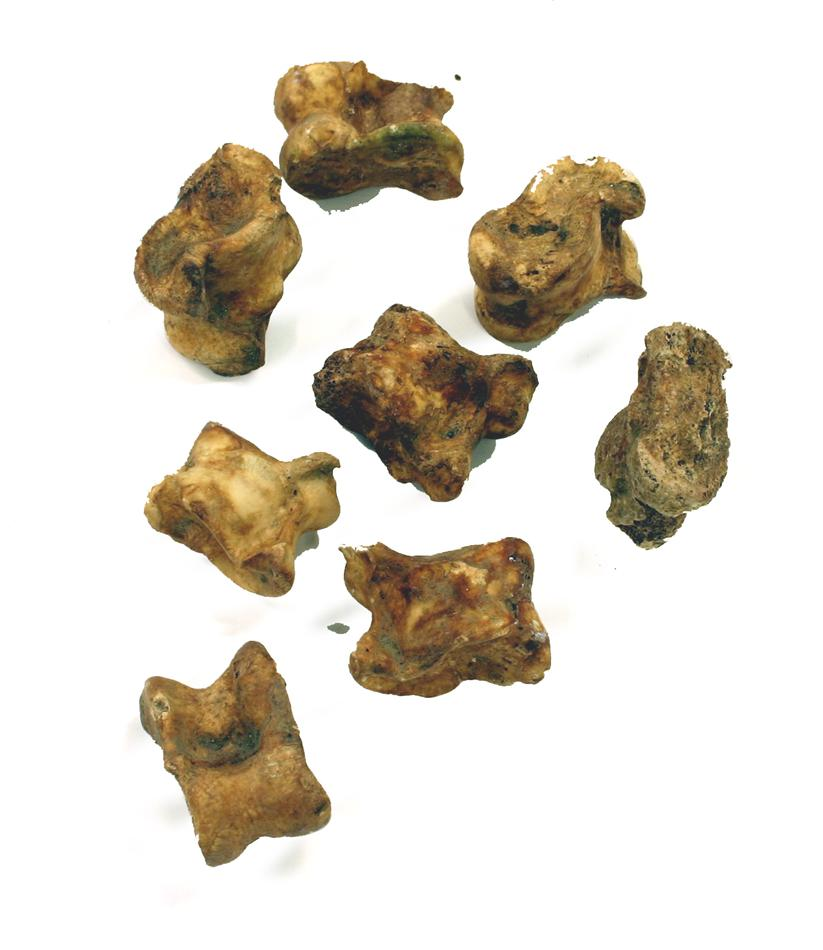
\includegraphics[width=0.5\hsize]{art/knucklebones.jpg}

%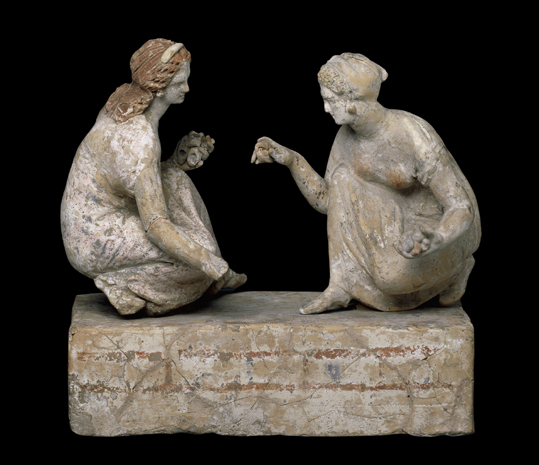
\includegraphics[width=0.8\hsize]{art/playing_knuckle_bones.jpg}
%\end{block}
%\end{column}
%\end{columns}
%\end{frame}


\begin{frame}
\frametitle{Purpose}
\begin{itemize}
    \item Many people like to argue about things.
    \item Usually they are not experts about those things.
    \item Maybe you are one of these people.
    \item I know I am.
    \item How can probability and statistics improve the outcomes of these
        arguments?
\end{itemize}
\end{frame}


\begin{frame}
\frametitle{The Speaker Reveals His Age}
    A conversation in 1993...
    \begin{itemize}
        \item \textbf{Bob:} Did you know that George Washington was the
            great-grandfather of Andrew Jackson?
        \item \textbf{Alice:} That's not true.
        \item \textbf{Bob:} It totally is!  Someone on Donahue was talking
            about it the other day.
        \item \textbf{Alice:} I'm pretty sure you're wrong, but that does
            sound like a reputable source...
    \end{itemize}
    An hour later
    \begin{itemize}
        \item \textbf{Alice:} Let's just agree to disagree.
    \end{itemize}
\end{frame}

\begin{frame}
\frametitle{Smartphones have Ruined Conversation}
    A conversation today...
    \begin{itemize}
        \item \textbf{Bob:} Did you know that George Washington was the
            great-grandfather of Andrew Jackson?
        \item \textbf{Alice:} That's not true.
        \item \textbf{Bob:} It totally is!  Someone posted it in the comments
            on a YouTube video.
        \item \textbf{Alice:} \textit{pulls up Wikipedia on her smartphone}
            According to this, Washington had no children.
        \item \textbf{Bob:} Damn you YouTube comments, how could you lead me
            astray\textinterrobang
    \end{itemize}

\end{frame}

\begin{frame}
\frametitle{This Conversation Is Over}
\begin{center}
    \frame{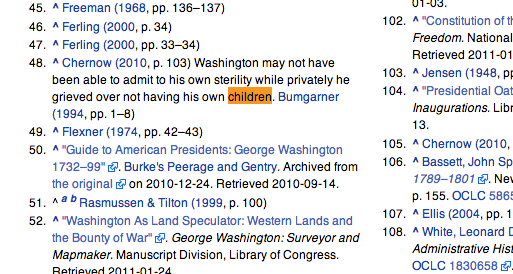
\includegraphics[width=\hsize]{art/washington_wikipedia.png}}
\end{center}
\end{frame}



\begin{frame}
\frametitle{Lightning Never Strikes Twice}
\begin{center}
    \frame{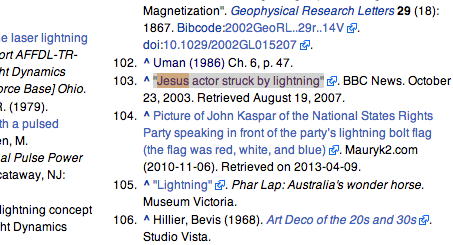
\includegraphics[width=\hsize]{art/lightning_wikipedia.png}}
\end{center}
The Point:  Some things are facts that can be looked up.
\end{frame}


\section{Damn Lies}

\begin{frame}
\frametitle{April Showers Bring May Flowers}
\begin{itemize}
    \item California dominates the US flower industry.
    \item \url{http://www.water.ca.gov} has detailed statistics on rainfall in
        California.
    \item US Department of Agriculture publishes the ``California Floricultural
        Report'' annually.
\end{itemize}
\end{frame}


\begin{frame}
\frametitle{}
\begin{center}
    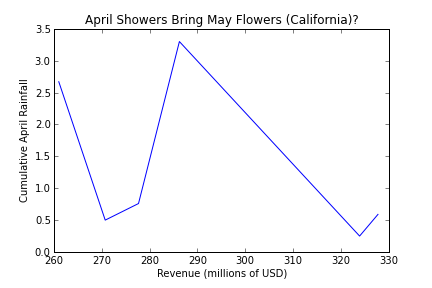
\includegraphics[width=\hsize]{art/april_showers.png}
\end{center}
\end{frame}

\begin{frame}
\frametitle{Everything Is on the Internet}
\begin{itemize}
    \item Find statistics on the thing(s) you care about.
        \begin{itemize}
            \item You'd be surprised what you can find statistics on.
            \item The trend is towards putting everything online.
        \end{itemize}
    \item Analyze them to see if your preconceived notion is correct.
\end{itemize}
\end{frame}


\section{Statistics}


\begin{frame}
    \frametitle{No Two Snowflakes Are
    Alike\footnote{\url{http://www.sultanik.com/blog/are-no-two-snowflakes-alike}}}
\begin{itemize}
    \item The shape of snow flakes can be decomposed into features.
    \item Approximately $10^{158}$ possible feature configurations.
        \begin{itemize}
            \item There are approximately $10^{80}$ atoms in the universe.
        \end{itemize}
    \item Approximately $(4.54 \times 10^9) * 10^{23} = 4.54\times 10^{32}$
        have fallen on the earth thus far.
    \item The probability of picking the same element twice when choosing
    $4.54\times 10^{32}$ elements from a set of $10^{158}$ is almost zero. 
    \item Maybe this saying has some truth to it!
\end{itemize}
\end{frame}


\begin{frame}
\frametitle{No Two Snowflakes Are
    Alike\footnote{Seriously, check out this post:  \url{http://www.sultanik.com/blog/are-no-two-snowflakes-alike}}}
\begin{itemize}
    \item Sultanik points out that the underlying assumption in the above
        analysis is that configurations are uniformly distributed.
    \item Some scientists think certain configurations are more likely than
        others (area of active research).
    \item If they follow a Zipfian or Normal distribution, and some simplifying
        assumptions are made, probability approaches one.
    \item If this seems unlikely, consider that with sixty people in a room, the
        probability that two share a birthday is almost one.
\end{itemize}
\end{frame}


\begin{frame}
\frametitle{Unique Snowflakes}
\begin{itemize}
    \item Example of back of the envelope calculations:
    \begin{itemize}
        \item Formulate the problem mathematically (hard part).
        \item Solve with math (easy part).
    \end{itemize}
\end{itemize}
\end{frame}

%------------------------------------------------


\begin{frame}
\frametitle{Your New Job:  Go Out There and Prove People Wrong}
\begin{center}
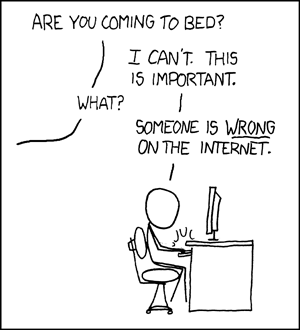
\includegraphics[height=0.8\vsize]{art/duty_calls.png}
\end{center}
\end{frame}


\end{document} 
